\section{Introduction}
\par Since its original proposal \citep{Cox1972}, Cox proportional hazards regression has become the most common regression approach for analyzing survival data.  Cox regression utilizes a partial likelihood construction under an assumption of proportional hazards to estimate the regression coefficients without having to specify the underlying baseline hazard.  The ability to avoid choosing a specific parametric distribution for the survival time is very attractive, as time-to-event data are often poorly described by fully parametric models.

This semiparametric flexibility, however, comes at a cost. The Cox regression approach can estimate relative risks, but without estimating the baseline hazard, it does not make any predictions concerning the absolute failure time for any given individual.  This poses a challenge to assessing the predictive accuracy of a given Cox regression model.  The challenge is particularly relevant for penalized Cox regression \citep{Tibshirani1997,Fan2002}, as the assessment of predictive accuracy via cross-validation is the standard method for selecting the regularization parameter and deciding upon a model.

\par Standard cross-validation involves dividing the data into $K$ folds, then fitting the model on $K-1$ of those folds (the training set) and assessing prediction accuracy on the remaining fold (the testing set). This process is then repeated, with each fold serving as the testing set exactly once. For Cox regression, the estimated coefficients allow us to quantify the risk for each subject in the training set relative to other members of the training set, but it is not obvious how to use those estimates to quantify the model's accuracy in the testing set.

\par One approach is to simply calculate the partial likelihood based on the observations in the test set as a measure for the model's predictive accuracy.  In doing so, we calculate the risk for each member of the test set relative to other members of the test set.  One drawback to this approach is that it becomes unstable when the size of the the test set is small.  In particular, it cannot be applied to leave-one-out cross-validation (LOOCV), as we must have at least two observations in the test set to compare their risk relative to each other.

%In this paper, we briefly review existing approaches for meeting this challenge, then propose two new methods for carrying out cross-validation in Cox regression models.

%As a semi-parametric model, Cox regression only gives estimations of the $\beta$ coefficients, without estimating the baseline hazard. Hence the interpretation of the Cox model is only valid in a relative sense.

% NOTE: I don't know that we need this paragraph; cross-validation is pretty common.
%One common approach for selecting the tuning parameter $\lambda$ for linear regression and logistic regression is via the K-fold cross validation. The data set would be split into K folds. One fold would be treated as the test set and the other K - 1 folds as the training set. The model would first be built on the training set, then fitted to the test set to obtain cross validation error (CVE).  CVE would be calculated for each candidate $\lambda$, then the one that minimizes cross validated error would be selected.

\par To overcome this drawback, an alternative approach was proposed by \citet{Verweij1993}.  Their approach, which we describe in detail in Section~\ref{Sec:cox-cv-existing}, stabilizes the cross-validated log likelihood, enabling its use even when the number of subjects in each fold is small.  This approach has been widely used and is implemented in R packages such as {\tt glmnet} \citep{glmnet}.  Although this approach fixes the stability issue, we demonstrate here that in practice, it tends to behave conservatively in terms of model selection.

\par In this paper, we propose two alternative ways to carry out cross validation for Cox regression. Instead of applying cross-validation to the partial likelihood directly, we propose applying cross validation to either the linear predictors of the regression model or to the deviance residuals \citep{Therneau1990}. Through simulation studies, we compare these proposed methods with existing cross-validation approaches for LASSO penalized Cox regression in both low- and high-dimensional settings.  \note{STILL TRUE?? We find that all cross validation approaches tend to be conservative,} but that the linear predictor approach offers the best combination of performance and stability, and we recommend using it for regularization parameter selection in penalized Cox models.  We conclude by applying both proposed and existing approaches to two high dimensional data sets from real studies with time-to-event outcomes.

%%%%%%%%%%%%%
%%%%%%%%%%%%%
\section{Methods}
%%%%%%%%%%%%%
%%%%%%%%%%%%%

\par In the Cox model, the hazard function for subject $i$ is given by 
\begin{equation*}
  h_{i}(t) = h_{0}(t) \exp( X_{i}^{T} \beta),
\end{equation*} 
where $h_{0}$ is the baseline hazard and $e^{X_i^{T} \beta}$ is the risk for a subject with covariates $X_i$ relative to that baseline.  The estimation of the coefficients is obtained by maximizing a partial likelihood.  Letting $t_i$ denote the time on study for subject $i$ and $\delta_{i}$ indicate whether or not an event is observed for subject $i$, each subject's individual contribution to that partial likelihood is
\begin{equation}
  \label{eq:cox-pl-subj}
  L_{i}(\beta) = \left \{\frac{\exp ( X_{i}^{T} \beta)}{\sum_{ k \in R(t_{i})}\exp ( X_{k}^{T} \beta)}\right \}^{\delta_{i}},
\end{equation}
where $R(t_{i})$ denotes the set of subjects at risk at time $t_{i}$.  The partial likelihood for the entire sample of $n$ subjects is then given by:
\begin{equation}
  \label{eq:cox-pl-sum}
  L(\beta) =\prod_{i = 1}^{n} L_{i}(\beta).
\end{equation}
Cox regression can be extended by introducing a penalty into the partial likelihood.  In penalized Cox regression, $\beta$ coefficient estimates are obtained by minimizing the objective function
\begin{equation}
  \label{eq:obj}
  Q(\beta) = - \frac{1}{n} \log L(\beta) + P_{\lambda}(\beta),
\end{equation}
where $P_{\lambda}(\beta)$ is a penalty function that depends on a regularization parameter $\lam$.

\par In this paper, we focus upon the LASSO penalty $P_{\lambda}(\beta) = \lambda \sum_{j} |\beta_{j}|$, although the methods we analyze can be used with any penalty as well as with model selection in unpenalized Cox regression (best subset selection). LASSO-penalized cox regression is particularly useful for high dimensional data where the number of covariates $p > n$; for example, in the prediction of overall survival in cancer patients based on genome-wide expression measurements. LASSO estimates yield a sparse model where some coefficients are estimated to be exactly zero. This sparsity pattern changes as we vary $\lam$: at large values of $\lambda$, most or all of the coefficients are 0, but as $\lam$ decreases, more covariates are selected. Selecting $\lambda$ is critical to LASSO estimation in the sense that the model's accuracy suffers if $\lam$ is either too large or too small.

\par Cross-validation is one of the most common methods used to select the appropriate $\lambda$ for penalized regression models. Suppose a data set $D$ of n observations is partitioned into $K$ folds: $D_{1}, D_{2}, \ldots, D_{K}$. For a given $k \in \left\{1,2,\ldots, K\right\}$, let $T_{k} = D - D_{k}$ denote the training set. This manuscript is concerned with the question: how should one use the $kth$ fold $D_{k}$ to measure predictive accuracy based on partial likelihood? In particular, the partial likelihood \eqref{eq:cox-pl-subj} involves a risk set -- which observations should be used to form that risk set?  In the following sections, let $L^{-k}$ denote the partial likelihood built over data in $T_k$, let $L^{k}$ denote the partial likelihood built over data in $D_k$, and $L$ denote the partial likelihood built over the entire data set $D$.  The log partial likelihood is denoted by $\ell$, with $\ell^k$ and $\ell^{-k}$ defined similarly. Finally, let $\hat{\beta}^{-k}$ denote the penalized estimates that are obtained by using $L^{-k}(\beta)$ in \eqref{eq:obj}.

%%%%%%%%%%%%%%%%%%%%
\subsection{Cross validated partial likelihood} 
\label{Sec:cox-cv-existing}
%%%%%%%%%%%%%%%%%%%%

\par A direct approach to measure a model's predictive accuracy in $D_k$ is to evaluate the log partial likelihood at $\hat{\beta}^{-k}$ using the data in $D_k$. Typically, cross-validation error (CVE) is measured by the total deviance across all $K$ folds, which (up to a constant) is given by:
\begin{equation}
  \label{eq:standard}
  \CVE = -2 \sum_{k=1}^{K} \ell^{k}(\hat{\beta}^{-k}).
\end{equation}
%where $\ell^{k}(\hat{\beta}^{-k}) = \sum \limits_{i \in D_{k}} \log L^{k}_{i}(\hat{\beta}^{-k})$.
We refer this approach as \emph{standard cross-validated partial likelihood}. This is implemented in the $\tt{glmnet}$ package as the \verb|"ungrouped"| option. \note{I added a -2 here so that CVE corresponds to deviance; this is what's done in glmnet/ncvreg}.

\par The standard approach is by far the most common way of conducting cross-validation for models such as linear regression and logistic regression. However, the standard approach can be problematic for Cox regression in the sense that that there may not be enough observations in $D_k$ to build up the risk set for partial likelihood. For example, the standard approach cannot work with leave-one-out cross-validation, since $\ell_k$ would either be zero or undefined for all folds.

To address this issue, \citet{Verweij1993} proposed an alternative method for cross-validation in Cox models:
\begin{equation}
\label{eq:VVH}
	\CVE = -\sum_{k = 1}^K \left\{ l(\hat{\beta}^{- k})  - l^{-k}(\hat{\beta}^{- k}) \right\}. 
\end{equation}
Here, $l(\hat{\beta}^{-k})$ is the log partial likelihood evaluated at $\hat{\beta}^{-k}$ using the entire data set $D$ and $l^{-k}(\hat{\beta}^{-k})$ is the log partial likelihood evaluated at $\hat{\beta}^{-k}$ on \note{FIX! the training set $T_k$. There should be enough observations in $T_k$ to build up the risk set as long as the entire data has a reasonable sample size.}  We refer to this cross-validation method as the Verweij and Van Houwelingen (V\&VH) approach. For many models, such as logistic regression or linear regression, these quantities $l(\hat{\beta}^{- k})  - l^{-k}(\hat{\beta}^{- k})$ and  $l^{k}(\hat{\beta}^{-k})$ are equivalent to each other -- in other words, the standard and V\&VH approaches agree.  However, Verweij and Van Houwelingen's approach is more stable for Cox regression as there is always a large number of observations in the risk sets its calculations are based on.  Since its proposal, the V\&VH approach has been widely implemented as a tool for cross-validation is Cox models.  For example, it is used by the R packages {\tt CoxRidge}, {\tt fastcox}, {\tt SGL}, {\tt CoxBoost}, {\tt mboost}, and {\tt glmnet} packages.  In {\tt glmnet}, it is the default choice for penalized Cox regression and is referred to as the {\tt grouped} option in the package's syntax.\note{PB: I like the mention of these packages, but they need citations.}

%%%%%%%%%%%%%%%%%%%%
  \subsection{Cross Validated Linear Predictors}
%%%%%%%%%%%%%%%%%%%%

\par Both of the methods in Section~\ref{Sec:cox-cv-existing} consist of adding together partial likelihood measures from each fold.  An alternative method is to obtain linear predictors for each fold, then combine these linear predictors to calculate a partial likelihood. We refer to this method as the \emph{cross-validated linear predictors} approach. To be more specific, we would first obtain $\hat{\beta}^{-k}$ from training set $T_{k}$; then the cross-validated linear predictors can be calculated for each observation $i$ from the test set $D_k$:  
\begin{equation}
  \label{eq:cv-lp}
  \hat{\eta}^{cv}_{i} = X_{i}\hat{\beta}^{-k}
\end{equation} 
After repeating this for all K folds, a complete set of cross-validated linear predictors $\hat{\eta}^{cv} = ( \hat{\eta}^{cv}_{1},  \hat{\eta}^{cv}_{2} , ...  \hat{\eta}^{cv}_{n})$ for the whole sample is obtained. A partial likelihood can then be built over this set of linear predictors to evaluate the predictive accuracy of the model: 
	\begin{equation} 
	L(\hat{\eta}^{cv}) = \prod_{i=1}^{n} \frac{exp (\hat{\eta}^{cv}_{i})}{\sum_{ j \in R(t_{i})}exp (\hat{\eta}^{cv}_{j})}.
	\end{equation}
\note{BIYUE: Throughout, use $\log$ instead of $log$, $\exp$ instead of $exp$, and $\ell$ instead of $l$.}
We define the cross-validation error evaluated with cross-validated linear predictors to be $$\CVE = - log L(\hat{\eta}^{cv}).$$
  
\par This idea of obtaining linear predictors over test sets, then constructing the partial likelihood after pooling all linear predictors together is implemented in R package \texttt{ncvreg} \citep{ncvreg}. This idea has also appeared in the cross-validation literature for quantities that cannot be evaluated on only a subset of the data, such as AUC in logistic and Cox regression models \citep{Parker2007,Simon2011a,Subramanian2011}.

  % \begin{figure}[h]
    %\centering
    %\begin{minipage}[b]{0.45\textwidth}
      %\centering
	%	  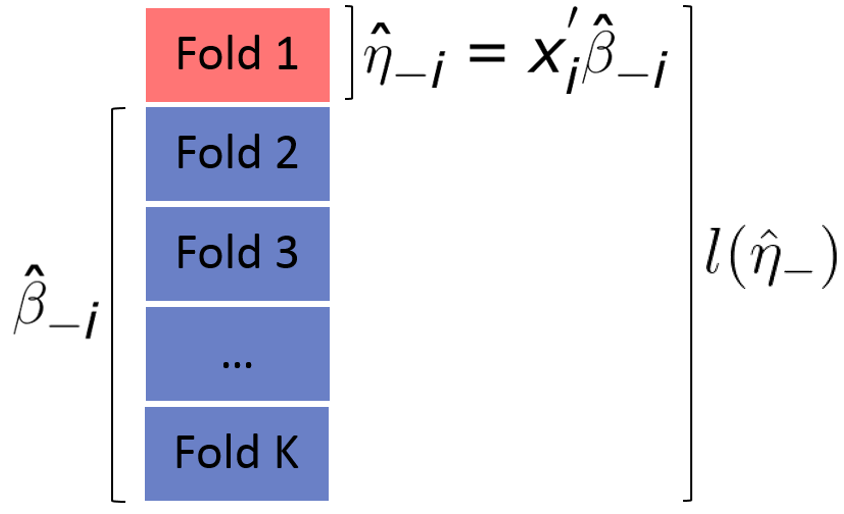
\includegraphics[height= 3.9cm ]{./figures/03.png}
      %\caption{CV Linear Predictors}
     %\end{minipage}
     %\begin{minipage}[b]{0.45\textwidth}
      %\centering
%		  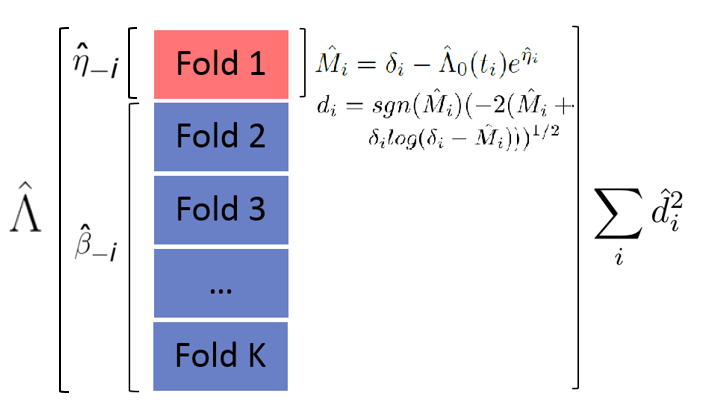
\includegraphics[height= 4.1cm ]{./figures/04_2.png}
    %  \caption{CV Deviance Residuals}
     % \end{minipage}	
  % \end{figure}	
    
%%%%%%%%%%%%%%%%%%%%
  \subsection{Cross Validated Deviance Residuals}
%%%%%%%%%%%%%%%%%%%%

The fundamental challenge of conducting cross validation for Cox regression is that the baseline hazard is not estimated from the model. Hence, another alternative approach to cross-validation would be to obtain an estimate $\hat{\Lambda}_{0}$ for the baseline hazard and use this in cross-validation.  There are several potential approaches to estimating $\Lambda_0$; in this manuscript, we chose to obtain the cross-validated linear predictors $\hat{\eta}^{cv}$ as in \eqref{eq:cv-lp}, then estimate $\Lambda_0$ via Kalbfleisch and Prentice's method \citep{Kalbfleisch2011}, treating these linear predictors as fixed inputs.\note{Maybe this isn't critical, but I still think we could just use $\hat{\Lambda}_0$ from the full data fit \ldots that estimator just makes more sense to me}

As an analogue to the residual sum of squares in linear regression, we considered using the sum of squared deviance residuals, the normalized form of Martingale residuals, to measure the model's predictive accuracy \citep{Therneau1990}. First proposed for model diagnostics, deviance residuals have also been used as a predictive accuracy measure in recursive partitioning models for survival data \citep{Therneau2018}. Given that the baseline hazard and linear predictors are obtained via cross-validation, we can first obtain the cross-validated Martingale residual: 
	\begin{equation}
	\hat{M^{cv}_{i}} = \delta_{i} -\hat{\Lambda}^{cv}_{0}(t_{i})e^{\hat{\eta}^{cv}_{i}},
	\end{equation} 
The cross-validated deviance residuals can then be derived from the Martingale residuals: 
	\begin{equation} 
	d_{i} = sgn(\hat{M}^{cv}_{i})\sqrt{-2(\hat{M}^{cv}_{i} + \delta_{i}log(\delta_{i} - \hat{M}^{cv}_{i}))}.
	\end{equation}
The sum of squared cross-validated deviance residuals, $\sum_{i}\hat{d}_{i}^2$ are used as the cross validated error. We refer to this method as the \emph{cross-validated deviance residuals} approach.

%A more straightforward way to compute the cross-validated deviance residuals is to estimate the baseline hazard using $T_k$, leaving $D_k$ as out-of-sample observations to calculate the residuals. There are two major issues with this approach. First, it is possible that some events in $D_k$ occurred after the last event in $T_k$. In this case, the survival function would drop to 0. Secondly, there is a numeric challenge for computing the term $log(\hat{\Lambda}_{0}(t_{i})e^{\hat{\eta}_{i}})$ in deviance residuals. Since the baseline hazard function is a step function from 0, the cumulative hazard $\hat{\Lambda}_{0}$ at the first time point from 0 is always 0. For whichever $D_k$ that contains the first time point, $log(\hat{\Lambda}_{0}(t_{i})e^{\hat{\eta}_{i}})$ would be negative infinity for that observation and lead to a numeric issue. To solve the first issue, events that occur later than the last event in $T_k$ should be censored. To solve the second issue, the step function of the baseline hazard needs to be smoothed. Both issues do not exist when the baseline hazard is built over the cross-validated linear predictors using all samples. \note{this paragraph may be optional, and can also be moved to discussion}

\begin{figure}
  \centering
		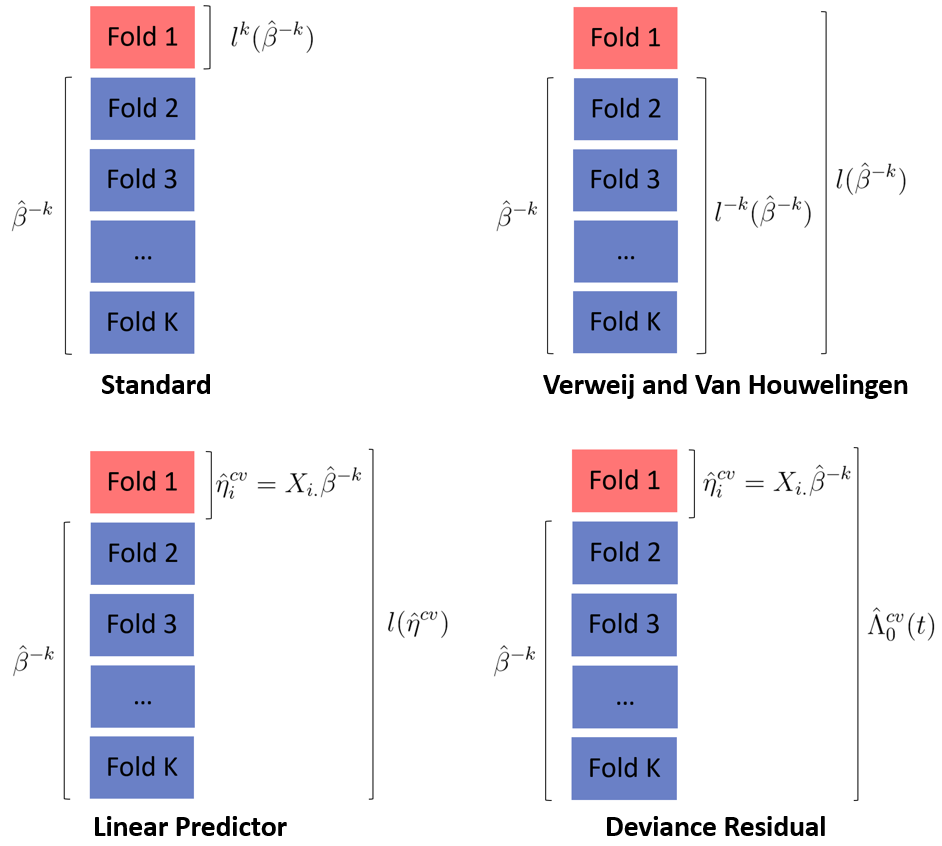
\includegraphics[height= 12cm ]{./figures/figure_1_new.png}
%		%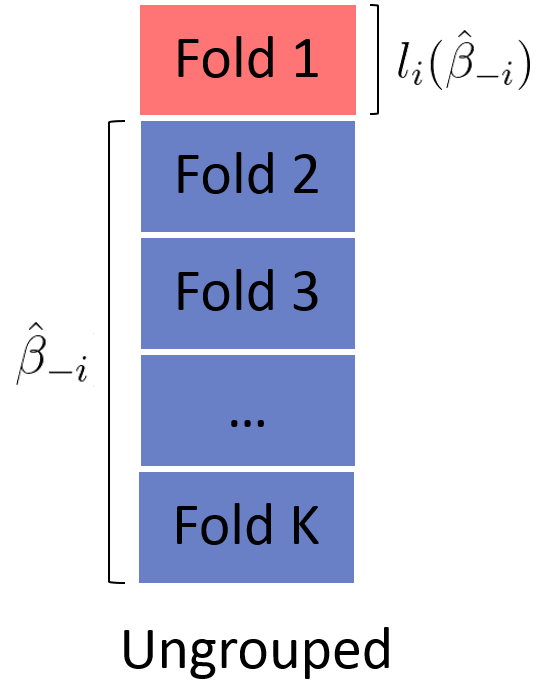
\includegraphics[height= 4cm ]{./figures/02_2.png}
   \caption{Illustration of K-fold Cross Validation Methods for Cox Regression}
\end{figure}	

%%%%%%%%%%%%%%%%%%%%
%%%%%%%%%%%%%%%%%%%%
\section{Simulation Studies}
%%%%%%%%%%%%%%%%%%%%
%%%%%%%%%%%%%%%%%%%%

Simulation studies were conducted to compare how those methods behave relative to each other in selecting the tuning parameter $\lambda$ and the corresponding model for LASSO penalized regression. Survival times were generated from exponential distribution $h(t) = h_{0} exp(X\beta)$, where $h_{0}$ is the prespecified baseline; $X$ is the covariate matrix generated from independent $Normal(0, 1)$ with $n$ observations and $p$ covariates; and $\beta$, the coefficients of the true model, is a vector whose majority entries are set to be 0 to guarentee sparsity. Censoring status were generated based on an independent binomial distribution. All simulations were implemented in R \citep{R}.

We first studied the accuracy of the models via several in-sample and out-of-sample measures. We varied the sample size, dimension, censoring percentage and signals of the simulated data sets to examine how those factors would affect the model selected via those cross-validation approaches. We also conducted a simulation study to examine the stability issue of the standard approach. Finally, we extended the comparison from K-fold cross-validation to Leave One Out Cross-validation (LOOCV).
   
%%%%%%%%%%%%%%%%%%%%%%%%%%%%%%%%
    \subsection {Simulations Comparing Predictive Accuracy}
%%%%%%%%%%%%%%%%%%%%%%%%%%%%%%%%
\par The first sets of simulation studies were conducted to study the predictive accuarcy of the model selected by the forementioned cross-validation approaches. We compared the predictive accuracy of the selected model via several distinct criteria.

\par We first measure the distance between the fitted model and the true model via mean squared error of the coefficients. Suppose $\hat{\beta}(\lambda)$ is the set of coefficients estimated by a cox model with LASSO penalty at $\lambda$. Mean squared error $MSE$ is defined to be 
\begin{equation}
E(\hat{\beta}(\lambda) - \beta)^2
\end{equation}
For each generated data set, an oracle model would be fitted using Cox regression only upon variables that are set as non-zero in the data generating process. The resulted estimates would be denoted by $\hat{\beta}^{oracle}$. Then the models selected by the cross validation methods with $\lambda^{cv}$ would be compared to the oracle model via 
\begin{equation}
log\left\{ \frac{MSE(\hat{\beta}(\lambda^{cv}))}{MSE(\hat{\beta}^{oracle})} \right\}
\end{equation}
for each cross-validation selected $\lambda^{cv}$ in each generated data set. The results would be averaged over N replications. We take $log$ of the MSE ratio to correct the right skewness.

%For each generated data set, the $\lambda$ that has the minimal MSE is chosen as the optimal $\lambda$, which we denote by $\lambda^{opt}$. Then the models selected by the cross validation methods with $\lambda^{cv}$ would be compared to the model that corresponds to $\lambda^{opt}$. We would take the ratio between $MSE$ of $\hat{\beta}(\lambda^{cv})$ and $MSE$ of $\hat{\beta}(\lambda^{optimal})$ for each cross-validation selected $\lambda^{cv}$ in each generated data set. The results would be averaged over N replications. 

\par We also measure the predictive accuracy via Brier score, which can be interpreted as the mean squared error of the prediction \citep{VanHouwelingen2011}. Suppose $\hat{S}(t_0|\lambda,x)$ is the prediction of survival probability of an individual beyond time $t_0$ with covariate $x$ based on model $\hat{\beta}(\lambda)$. Suppose the actual observation is defined as $y = \mathbb{1}(\left\{ t > t_{0}\right\})$, which is an indicator of whether the event is observed after $t_0$ or not. Then the Brier score is defined to be:
\begin{equation}
	Brier(y, \hat{S}(t_0|\lambda,x)) = (y - \hat{S}(t_0|\lambda,x))^2
\end{equation}
In our simulations, for each generated data set, we generated another independent data set that has 1000 observations without censoring. We computed Brier Scores upon all individuals in this independent test set where $t_0$ is set to be the median survival time for all four models selected by cross-validation. Lower Brier Scores means smaller prediction error, thus indicating better prediction accuracy.

\par The third measure we used is the Kullback-Leibler score, which measures the log-likelihood of the prediction model evaluated at the observations \citep{VanHouwelingen2011}. With the same notation defined in the previous paragraph, the Kullback-Leibler score is defined to be:
\begin{equation}
	KL(y, \hat{S}(t_0|\lambda,x)) = -\left\{ ylog(\hat{S}(t_0|\lambda,x) + (1 - y)log(1 - \hat{S}(t_0|\lambda,x)) \right\}
\end{equation}
We computed KL score upon individuals in the independent test set at their median survival time for all four models selected by cross-validation. Results were then averaged over the N replications. Lower KL Scores means smaller discrepency between the selected model and the true model, thus indicating better prediction accuracy.

\par While the MSE, Brier Score and Kullback-Leibler Score are good measures of the model, they are not very interpretable. Hence, we included Harrell's C Index as the last measure of the predictive accuracy\citep{HarrellJr1984}. The C Index is a rank-based statistic that measures the concordance between the linear predictor of the selected model and the observed outcome. Suppose we arbitrarily take two observation out of the data. If the observation that has a greater prognostic score also has a greater risk or shorter survival time until the event occur, then this would be considered as a concordant pair. C Index estimates of proportion of concordance pairs in the data set. C Index of 0.5 means the prediction is as good as flipping a coin and C Index of 1 means perfect concordance. We also computed Harrell's C Index upon the independent test set for all four models selected by cross-validation and averaged over all replications.

The simulation experiments were first conducted when the signal in the data was varied. In each simulated data set, there are n = 120 observations and p = 1000 covariates. 10$\%$ of the observations were censored. 10-fold cross-validation was implemented for all four methods. Number of non-zero $\beta$s was 10. The signal in the data set was varied by varying the magnitude of the $\beta$s from 0.4 to 0.9. For each scenario, 200 replications were used. 
   
\begin{figure}[h]
    \centering
		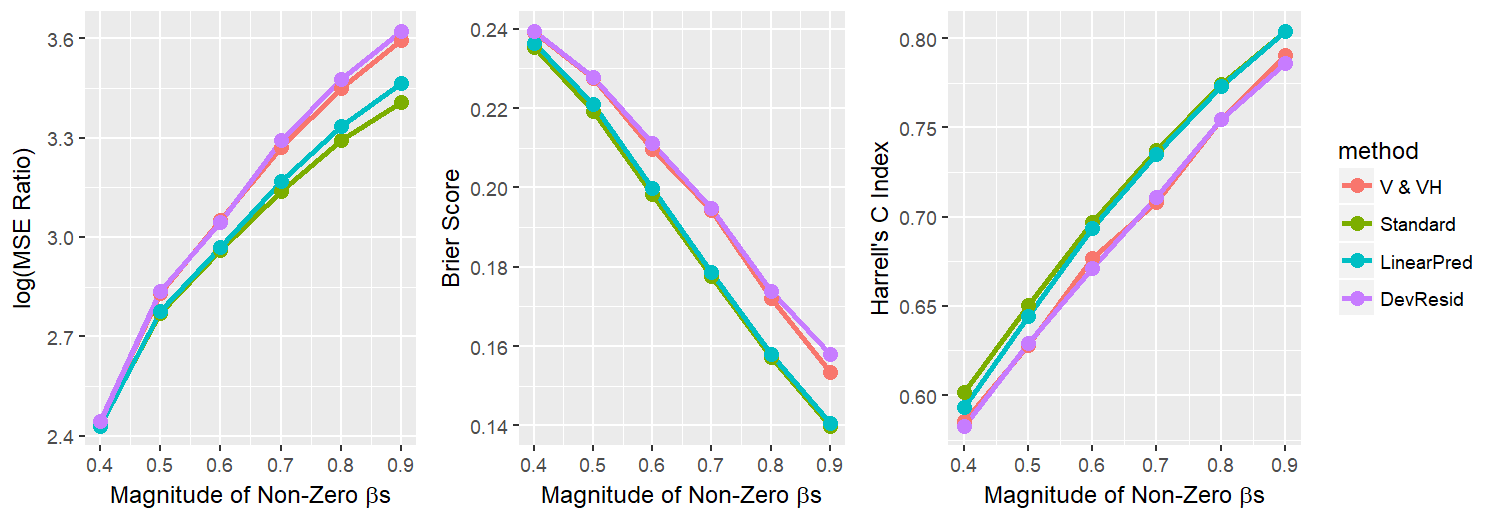
\includegraphics[height= 7cm ]{./figures/figure_2_new.png}
    \caption{Simulation Studies Comparing 4 CV methods in terms of $\lambda$ and MSE ratio. n = 150, p = 1000, 10$\%$ censoring.}
\end{figure}	

%The left panel compares the $\lambda$ selected by different methods. Verweij and Van Houwelingen's cross-validated partial likelihood approach, which is currently most widely used approach, consistently selects $\lambda$s that are greater than the optimal one.  Greater $\lambda$ leads to greater penalties and fewer non-zero variables, hence Verweij and Van Houwelingen's approach is conservative in terms of selecting variables. While the proposed cross-validated Deviance residual has very close performance as Verweij and Van Houwelingen's approach, the standard cross-validated log likelihood and the cross-validated linear predictor were more liberal than the other two methods. In general, all four methods tends to act conservatively and selects smaller models. 

\par Results of the simulation were illustrated in Figure 2. The x axis of the plots are the magnitude of the non-zero $\beta$ coefficients. The left panel compares the MSE ratios of selected models.  The y-axis represents the MSE ratios between the cross-validation selected models and the oracle model. The standard method has the smallest MSE ratio. The linear predictor approach's performance is also very close the standard approach. Both Verweij and Van Houwelingen's approach and the proposed deviance residual approach yield models that have greater MSE. The middle panel compares the Brier scores of the models selected. The y-axis represents the Brier score. The standard method and the linear predictor approach have lower brier score across all levels of signals. Both Verweij and Van Houwelingen's approach and the proposed deviance residual approach yield models that have greater Brier scores. The left panel compares Harrell's C of the models selected. The y-axis represents Harrell's C, which increases from around 0.6 to 0.8 as the coefficent size increases. The standard method and the linear predictor approach have slightly higher Harrell's C across all levels of signals, indicating better prediction accuracy. Overall, all four methods have very close performance . 
 
\begin{table}[h]

\setlength{\tabcolsep}{3pt}

\caption{\label{tab:} Simulation Studies that Compare All Four Cross-Validation Methods Varying Dimension and Signal }
\centering
\begin{tabular}[t]{cccccccccc}
\toprule
 n& p& $\#$ Non-Zero & Signal & Method & $\lambda$ & log(MSE Ratio) &Brier Score & Kullback Leibler & C Index\\
\midrule
150 & 50 & 5 & low & V VH  & 0.095 (0.028) & 1.457 (0.954) & 0.242 (0.013) & 0.678 (0.029) & 0.617 (0.034) \\
    &    &   &     & Standard  & 0.087 (0.030) & 1.459 (0.922) & 0.242 (0.013) & 0.678 (0.029) & 0.618 (0.032) \\
    &    &   &     & LinearPred  & 0.088 (0.025) & 1.433 (0.927) & 0.241 (0.013) & 0.677 (0.028) & 0.620 (0.029) \\
    &    &   &     & DevResid  & 0.132 (0.032) & 1.676 (1.019) & 0.248 (0.014) & 0.689 (0.030) & 0.601 (0.044) \\
\addlinespace
150 & 50 & 5 & strong & V VH  & 0.070 (0.011) & 1.733 (0.922) & 0.177 (0.012) & 0.527 (0.030) & 0.750 (0.014) \\
    &    &   &     & Standard  & 0.066 (0.012) & 1.688 (0.909) & 0.176 (0.012) & 0.526 (0.029) & 0.749 (0.014) \\
    &    &   &     & LinearPred  & 0.067 (0.011) & 1.695 (0.925) & 0.176 (0.012) & 0.526 (0.030) & 0.750 (0.014) \\
    &    &   &     & DevResid  & 0.110 (0.012) & 2.339 (0.868) & 0.187 (0.014) & 0.554 (0.033) & 0.750 (0.018) \\
\addlinespace
300 & 10000 & 20 & low & V VH  & 0.139 (0.021) & 3.463 (0.438) & 0.244 (0.015) & 0.681 (0.032) & 0.612 (0.051) \\
    &    &   &     & Standard  & 0.105 (0.027) & 3.350 (0.458) & 0.228 (0.021) & 0.646 (0.045) & 0.639 (0.05) \\
    &    &   &     & LinearPred  & 0.107 (0.026) & 3.360 (0.462) & 0.229 (0.021) & 0.648 (0.045) & 0.638 (0.049) \\
    &    &   &     & DevResid  & 0.139 (0.027) & 3.454 (0.447) & 0.243 (0.018) & 0.678 (0.038) & 0.610 (0.058) \\
\addlinespace
500 & 10000 & 20 & strong & V VH  & 0.072 (0.005) & 3.469 (0.480) & 0.162 (0.015) & 0.495 (0.036) & 0.784 (0.021) \\
    &    &   &     & Standard  & 0.056 (0.005) & 3.174 (0.504) & 0.153 (0.011) & 0.465 (0.029) & 0.782 (0.017) \\
    &    &   &     & LinearPred  & 0.057 (0.005) & 3.204 (0.498) & 0.153 (0.011) & 0.466 (0.029) & 0.783 (0.017) \\
    &    &   &     & DevResid  & 0.076 (0.005) & 3.545 (0.467) & 0.167 (0.015) & 0.508 (0.035) & 0.782 (0.022) \\
\bottomrule
\end{tabular}
\end{table}

\par Additional simulation studies were conducted for other four scenarios, which are a combination of different dimensions and signal in the data. The results are shown in Table 1. More specifically, we examined low dimension (p = 50) with weak signal, low dimension with strong signal, high dimension (p = 10000) with weak signal and high dimension with strong signal. Censoring was set to be 30$\%$. Overall, the standard approach and linear predictor approach tend to select smaller $\lambda$ and select more variables than the other two approaches. Among all four of them, the Deviance residual approahc is the most conservative one.

\par Scenarios with higher signal and lower dimensions are considered as easier scenarios to select the most predictive model. As is shown in the results, at p = 10000 with weak signal, which is the hardest scenario, the standard approach and the linear predictor approach have the greatest advantage. They out-performed the other two methods in all predictive measures. The differences in performance are neglegible at low dimension or when there is strong signal in the data.

\subsection {Stability}
  
\par In this section, simulation studies were conducted to address the stability issue of the standard cross-validated likelihood. The standard approach is the most straighforward among all four methods that are presented in this paper. It also has the best predictive accuracy based on the simulation results in the previous section. However, this approach is much less widely used due to its unstability. When number of observed events in $D_k$ is really small, there would be insufficient number of events to construct the risk set for the partial likelihood. We thus conducted a simulation study varying the number of folds and censoring to see when the method would start to have convergence issue. In both studies, we set the number of observations to be n = 100. When we varied the censoring percentage, we fixed the number of folds K = 10; when we varied the number of folds, we fixed the censoring to be 10$\%$. N = 200 replications were used to estimate the convergence probability.
\par As is illustrated in Figure 3,  the standard approach start to have converge issue fairly quickly when censoring increases or when the number of folds increases. While the linear predictor approach performs as well as the standard approach in terms of prediction accuracy, the linear predictor approach is also as stable as the Verweij and Van Houwelingen's approach.

\begin{figure}[h]
    \centering
		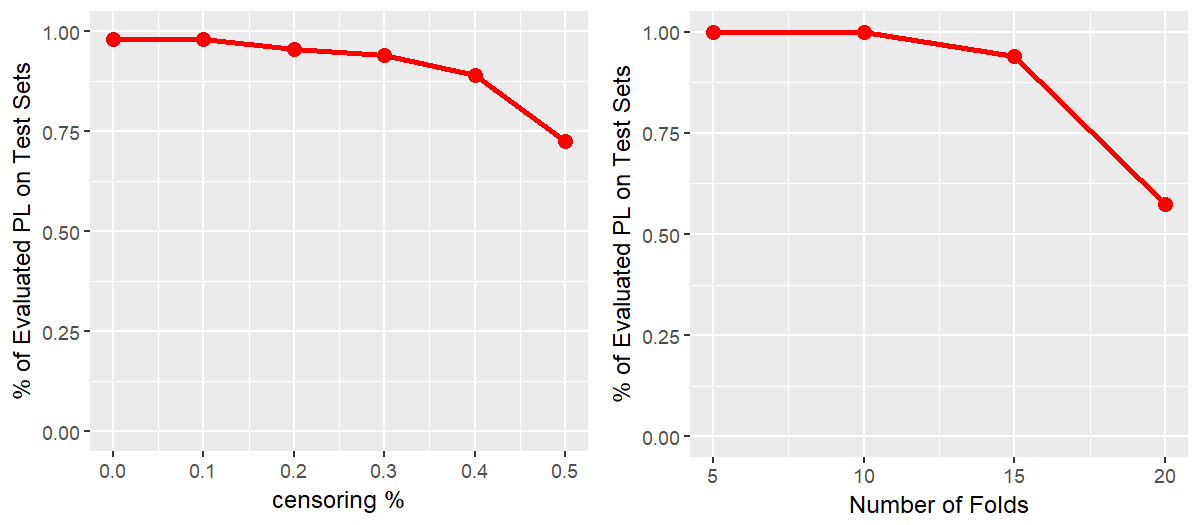
\includegraphics[height= 7cm ]{./figures/figure_3_new.png}
    \caption{Comparing Stability}
\end{figure}	

    \subsection {Leave-One-Out Cross Validation}
	\par In this section, we compared Leave-One-Out Cross Validation (LOOCV) with 10-fold cross validation. When first introduced, Verweij and Van Houwelingen's cross-validated partial likelihood was proposed so that LOOCV for Cox regression became feasible. While Verweij and Van Houwelingen's cross-validated partial likelihood solves the stability issue by aggregating more observations together, it does not seem to be an efficient way to evaluate the model fit based on results in Section 3.1. It tends to be conservative in variable selections and selects fewer variables in various scenarios. We further examined Verweij and Van Houwelingen's cross-validated partial likelihood under Leave-One-Out Cross Validation. In the following simulation studies, we used 10 fold cross-validated standard approach as our baseline for comparison. Then we conducted both 10-fold CV and LOOCV for Verweij and Van Houwelingen's approach, linear predictor approach and deviance residual approach.
	\par Results of the simulation experiment is illustrated in Figure 4.For all three methods, LOOCV selected models that have smaller MSE than 10-fold CV for all three CV approaches. As is shown in left and middle panels, LOOCV based on deviance residuals and Verweij and Van Houwelingen's cross-validated partial likelihood still perform more conservatively than the standard approach. Even if Verweij and Van Houwelingen's approach was proposed to allow LOOCV, the LOOCV based on Verweij and Van Houwelingen's approach does not surpass the 10-fold standard approach.

    %\par We also compared cross-validation with information criteria AIC and BIC. Simulation studies were conducted in lower dimension and higher dimension respectively. As is illustrated in Figure 7, in lower dimension, AIC tends to perform more liberal and BIC tends to perform more conservative than the optimal $\lambda$. While the cross-validation methods are also conservative, most of them are less conservative than BIC. In terms of MSE, cross-validation methods yield smaller MSE than the information criteria. In higher dimension, both BIC and AIC tend to be more liberal than the optimal $\lambda$ and yield larger MSE.

\begin{figure}[h]
    \centering
		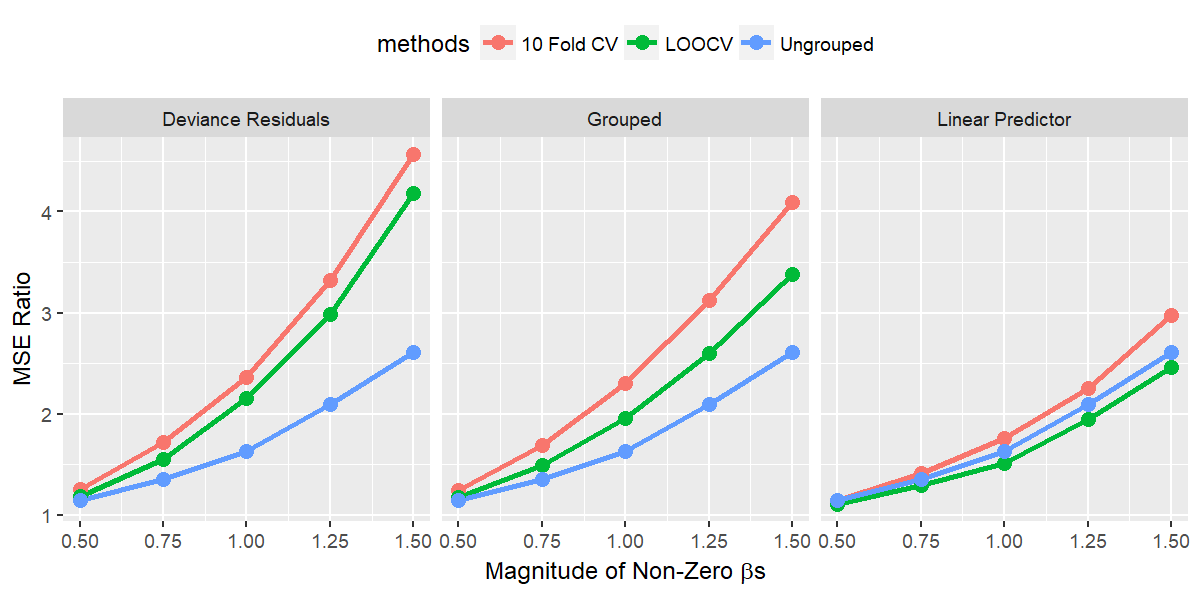
\includegraphics[height= 8cm ]{./figures/figure_4.png}
    \caption{LOOCV}
\end{figure}	

  %\subsection {Simulations on Deviance Residuals and Baseline Hazard Estimations}

 \subsection {Cross-Validated C Index}
\par In this section, we conducted simulation experiments to compare likelihood-based cross validation against AUC-based cross validation. While the focus of this manuscript is to study valid cross-validation methods for partial-likelihood-based models such as penalized Cox rgression, the methods proposed in this paper are not applicable to some other survival machine learning models that do not involve constructing a partial likelihood. In those cases, the cross-validated C Index, also called cross-validated AUC, is one of the most popular options \citep{Subramanian2011} \citep{Simon2011a}. As is proposed by Simon et al., cross-validated AUC is computed also based on cross-validated linear predictors or some other types of prognostic factors. Thus, it is of our curiosity to see which one has a better performance when those two approaches, likelihood-based and AUC-based, are both available after we obtain the cross-validated linear predictors.

\par We conducted simulations at both low dimension (p = 50) and high dimension (p = 1000), varying the signal in the data. Results of the simulations are illustrated in Figure 5. In general, the likelihood-based approach is more stable than the AUC-based cross validation approach. For MSE ratio and Brier Score, the likelihood approach tends to select more predictive models than the AUC-based approach. For the actual $\lambda$, it is interesting that the AUC-based approach is quite liberal and selected smaller $\lambda$s, which would yield models that contain more variables. 

\begin{figure}[h]
    \centering
		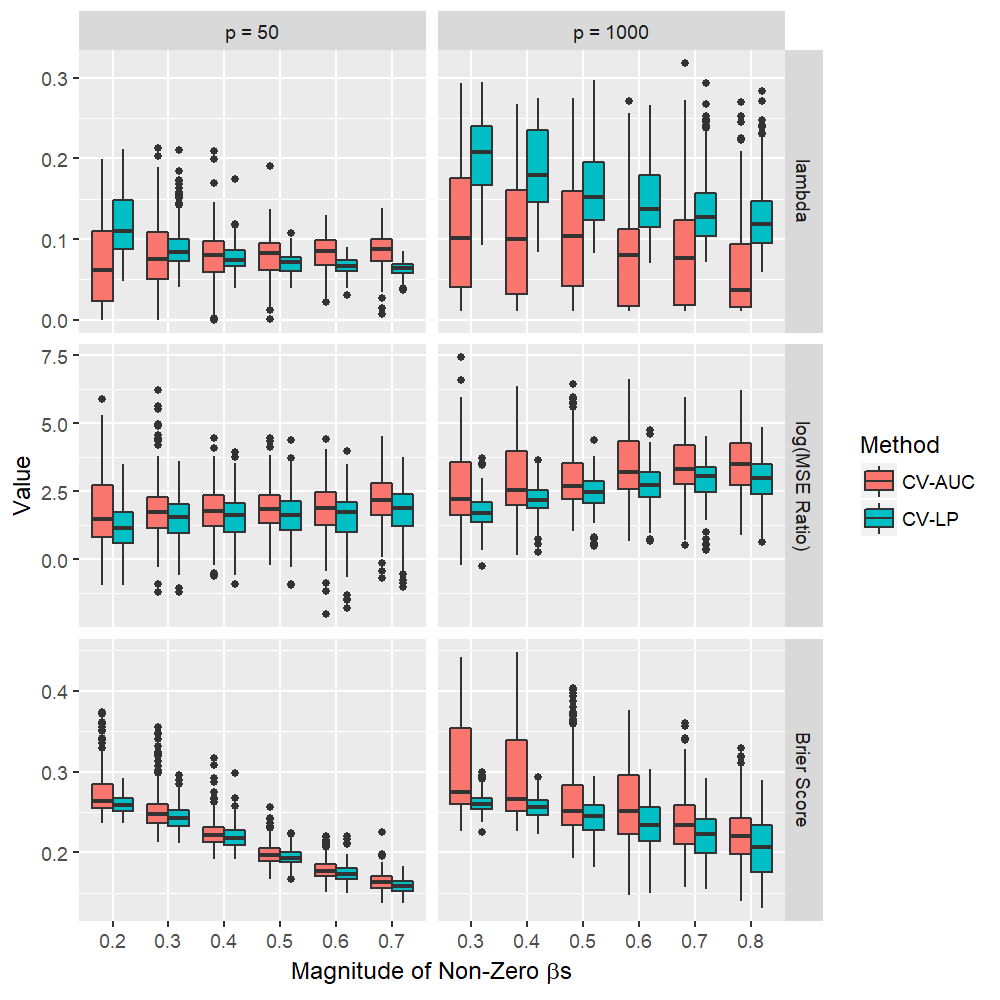
\includegraphics[height= 15cm ]{./figures/figure_auc.png}
    \caption{Cross-Validated AUC}
\end{figure}	

\begin{figure}[h]
    \centering
		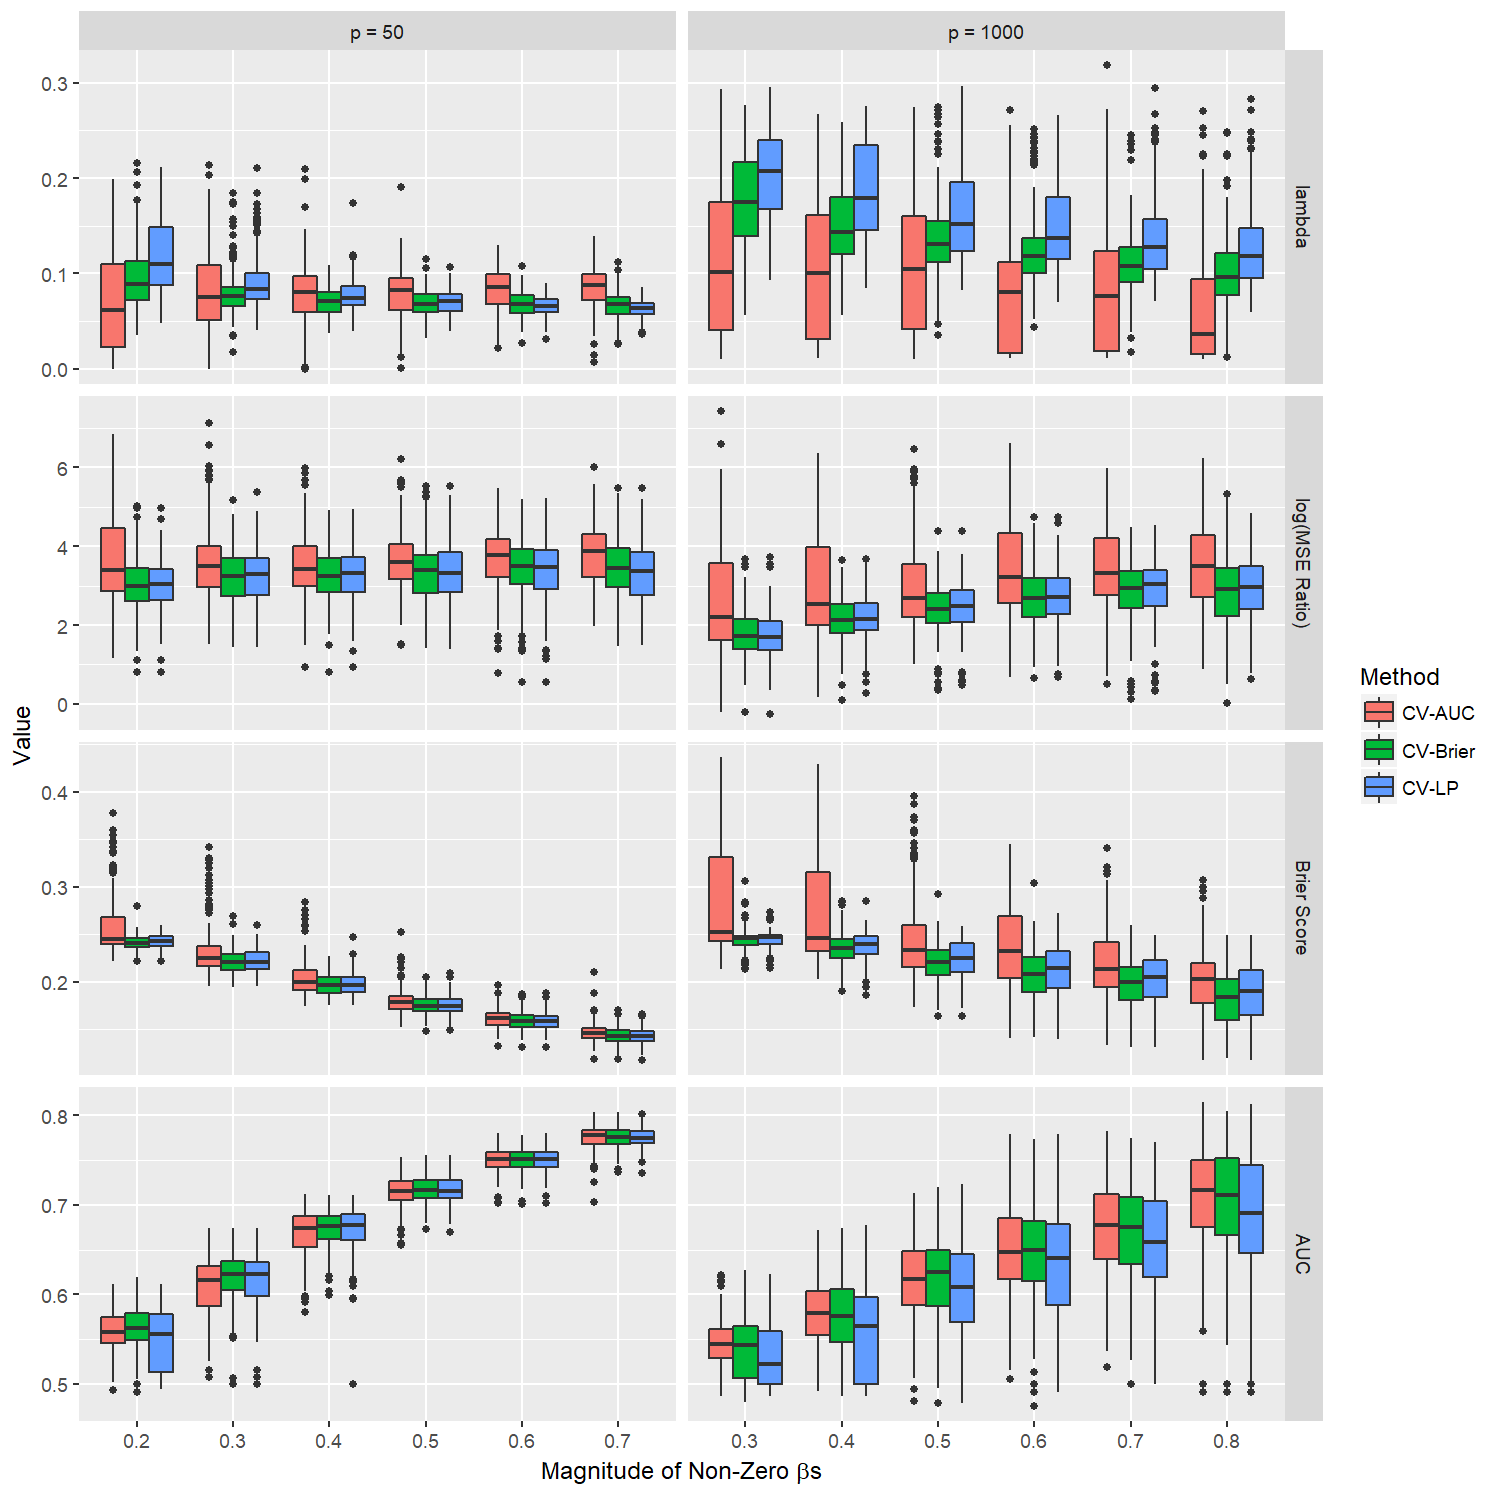
\includegraphics[height= 15cm ]{./figures/figure_auc_extended.png}
    \caption{Cross-Validated AUC}
\end{figure}	

\section{Application to Real Data}

\par In this section, we compared the performances of those cross validation methods when they are applied to data from real lung cancer study. \cite{shedden2008gene} conducted a large, retrospective study to validate prognostic gene expression signatures as predictors of overall survival in lung cancer patients, They performed gene expression profiling of \textit{442} non-small-cell lung cancer (NSCLC) patients. The data set contains gene expression measures from \textit{22,283} genes and basic clinical variables such as stage, age and gender. 236 death events were observed and about 50$\%$ of the patients are censored. The clinical variables stage, age and gender were known to have a larger prognostic impact, thus they were fitted in the model without penalization. Cross-validation was again used for the selection of the penalty term, which selects the gene expressions that are associated with patients' overall survival. The results of the analysis are also listed in Table 3.

\par How the CV methods perform on real data reflects what is shown in simulation studies. The standard CVE is the most liberal approach. Deviance Residual and Verweij and Van Houwelingen's CVE approaches were both really conversative, while the standard approach was the second liberal to standard CVE. In Figure 5, the Cross Validated Error is rescaled and plotted for all four methods. A $\lambda$ will be selected when CVE curve reaches its lower point. The blue line, which represents the linear predictor approach, has more curvature near its lowest point. It is easier to pick out the minimum point for this blue curve. Hence this approach is better at picking out signals than the other three approaches. For Verweij and Van Houwelingen's cross-validated partial likelihood, there's almost no signal there.

\begin{figure}[h]
    \centering
		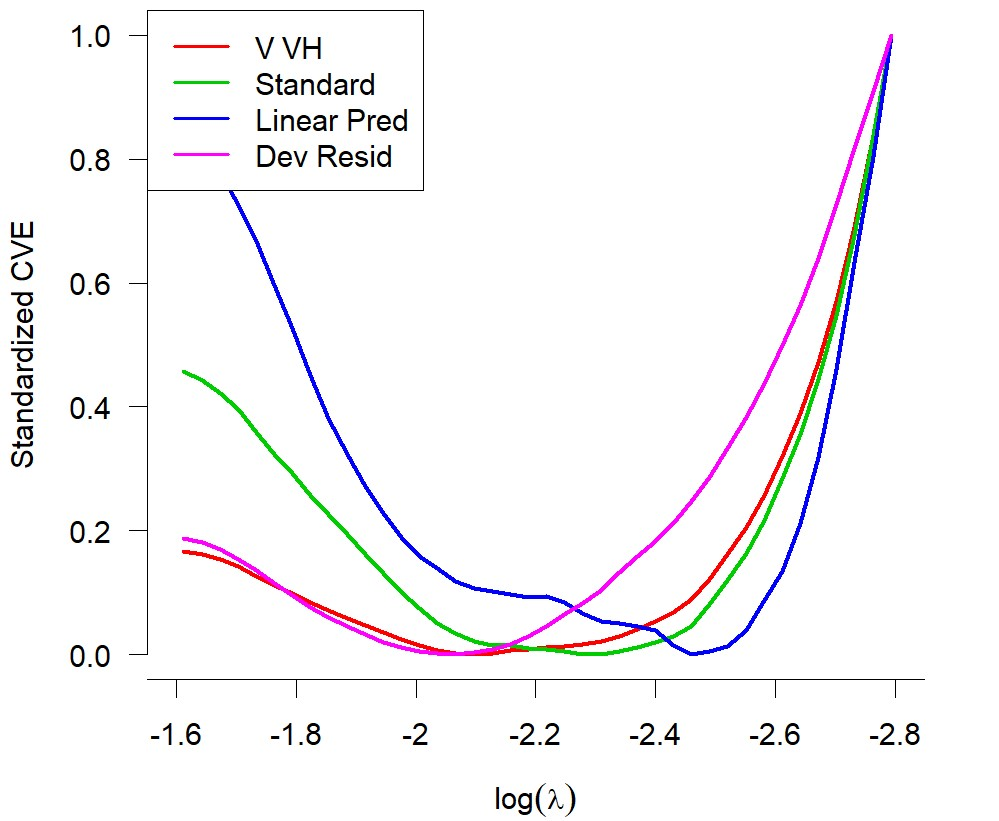
\includegraphics[height= 8cm ]{./figures/shedden.jpg}
    \caption{Comparing Cross-Validated Error for Different Methods on Real Data Sets}
\end{figure}	

\begin{table}[h]
\centering
\caption{Application to Real Data Sets}
\label{my-label}
\begin{tabular}{lccccc}
\toprule
						& $\lambda$ & log($\lambda$) & CV AUC & Brier Score \\ 
						\cline{2-5} \\ 
						V $\&$ VH& 0.123 & -2.097 & 0.640 & 0.246\\
						standard & 0.102 & -2.278 & 0.643& 0.239\\
						Linear Pred &0.085 & -2.460 & 0.651&  0.227\\
						Dev Resid & 0.127& -2.066 & 0.639& 0.246\\ 
						\bottomrule
\end{tabular}
\end{table}

\section{Discussion}

\par Four methods of conducting cross-validation for Cox Regression were compared through simulation studies in terms of their predictive accuracy. All cross-validation methods tend to select the more conservative model: with greater value of $\lambda$, and fewer variables selected into the model. Despite of the stability issue, the standard approach is the most liberal one across all scenarios and yield the least MSE. The proposed linear predictor approach performs closely to the standard approach. Under LOOCV, the linear predictor approach out-performs the standardstandard approach. Both Verweij and Van Houwelingen's approach and the proposed Deviance Residual approach perform conservatively, hence not recommended for use in practice. Results from real data application reflects results from the simulation studies.

% Discussion on Deviance Residual

%\par While the Deviance Residual approach has a reasonable performance in scenarios where dimension is high, it tends to act more conservatively than all the other three approaches in general. As is noted by Therneau et al, the sums of squared martingale residuals and deviance residuals do not necessary reflect how good the model fit is \citep{Therneau2000modeling}. The difficulty of estimating the baseline hazard seems to play an important role. A series of simulations were thus designed to study how baseline hazard estimation affects the deviance residuals' performance as a measurement for model fit. 

%\par In the following simulation studies, the defined optimal $\lambda$ and the $\lambda$ selected by the Linear Predictor approach were used as benchmarks. Various sample sizes and dimensions were varied. The survival outcomes were generated both from exponential distribution and Weibull distribution. Six different approaches were compared in terms of baseline hazard estimation and their impact on sums of squared deviance residuals. Two non-parametric approaches, Kalbfleisch and Prentices' estimator and Breslow's estimator, were used first for estimating the cumulative hazard baseline \citep{Kalbfleisch2011} \citep{breslow1972}.  As is presented in column 3 and column 5 in Table 2, the sum of squared deviance residuals computed based on both approaches are all very conservative compared to the optimal $\lambda$. Their performance is extremely bad when n is large and p is small. 

%\par Since both of the non-parameteric estimations seemed to perform well at early time points but poorly later, a weighted approach was then applied to emphasize earlier time points. Weights are assigned proportional to number of subjects at risk, making earlier time points weighted more than later time points. Results of these two approahces are presented in column 4 and 6 in Table 2. The attempt to improve the non-parameteric estimations via weighting does not seem to improve the selection too much. 

%\par In the next step,  the non-parametric baseline hazard estimation was replaced by the exact baseline hazard that was used to generate the outcome. Results were listed in the seventh column in Table 2. When the baseline was known, the performance of sum of squared deviance residuals actually performed really close to the optimal $\lambda$. This simulation suggests that when the baseline hazard was accurately estimated, then the sum of squared deviance residuals gave really good measures for the model fit.

%\par In the last step, we replaced the non-parametric baseline hazard estimation with a parametric approach, where we assume the baseline hazard to follow an exponential distribution. We derived the estimation for baseline hazard by maximum likelihood approach conditioned on covariates: $\hat{\lambda}_{0} = \frac{\sum d_{i}}{\sum t_{i}e^{\eta_{i}}}$. The results are listed in the eighth column in Table 2. When this estimation was used for data that were generated from exponential distribution, its performance was as well as when the exact baseline was specified. When it was fitted to data that were generated from the Weibull distribution, that is when the model is misspecified, then its performance was even worse than the non-parametric approaches.

%\par Hence, getting accurate estimation of the baseline hazard is crucial to whether or not the sum of squared deviance residuals can be a good measurement for model fit.

%\begin{table}[h]
%	\small
%	\caption{Average of Selected $\lambda$ with Different Baseline Estimation for Deviance Residuals}
	%\centering
	%\begin{tabular}{lllllllll}
	%\hline
	%\\[-0.75em]
    %& Optimal & Linear Pred & KP & KP & Breslow & Breslow & Exact & Exp\\ 
    %&  & & & weighted & & weighted & & \\ \cline{2 - 9} 
	%\textbf{True Baseline: $Exponential(1)$} &&&&&&&&\\
	%n = 100, p = 10, non-zero $\beta$: 2 & 0.0461 & 0.0665 & 0.1986 & 0.1970 & 0.1908 & 0.1975 & 0.0540 & 0.0539 \\
	%n = 100, p = 100, non-zero $\beta$: 20 &0.0555 & 0.1841 & 0.2359 & 0.2201 & 0.2146 & 0.2244 & 0.0805 & 0.0985 \\
	%n = 100, p = 1000, non-zero $\beta$: 20 & 0.0268 & 0.0505 & 0.0948 & 0.0798 & 0.0867 & 0.0809 & 0.0288 & 0.0270 \\
	%\textbf{True Baseline:} $Weibull$ &&&&&&&& \\
 	%n = 100, p = 10, non-zero $\beta$: 2 & 0.0476 & 0.0710 & 0.2004 & 0.1969 & 0.1907 & 0.1907 & N/A & 0.2330 \\ 
	%\hline
%\end{tabular}
%\end{table}


\section{Appendix}

\begin{figure}[h]
	\centering
	\begin{minipage}[t]{10cm}
	\begin{algorithm}[H]
	\caption{Standard Method}
	\par \For{k in 1 to K } 
	{
		 Fit Cox Regression on $T_{k}$: Obtain model estimates $\hat{\beta}^{-k}$\;
		 Evaluate the partial likelihood of $\hat{\beta}^{-k}$ on $D_{k}$: $l^{k}(\hat{\beta}^{-k})$\;		
	} 
	
	\par $ CVE_{st} = - \sum_{k = 1}^{K} l^{k}(\hat{\beta}^{-k})$
 	\end{algorithm}

	\begin{algorithm}[H]
  	 \caption{Verweij and Van Houwelingen's Method}
	\par \For{k in 1 to K } 
	{
		 Fit Cox Regression on $T_{k}$:  Obtain model estimates $\hat{\beta}^{-k}$\;
		 Evaluate the partial likelihood of $\hat{\beta}^{-k}$ on $T_{k}$: $l^{-k}(\hat{\beta}^{-k})$\;
		 Evaluate the partial likelihood of $\hat{\beta}^{-k}$ on $D$: $l(\hat{\beta}^{-k})$\;
		 Take the difference: $ l(\hat{\beta}^{-k}) - l^{-k}(\hat{\beta}^{-k}) $\;
	} 

	\par $ CVE_{vvh} = - \sum_{k = 1}^{K} \left\{ l(\hat{\beta}^{-k}) - l^{-k}(\hat{\beta}^{-k}) \right\}$
	\end{algorithm}

	\begin{algorithm}[H]
    	\caption{Cross-Validated Linear Predictors}
	\par \For{k in 1 to K } 
	{
		 Fit Cox Regression on $T_{k}$:  Obtain model estimates $\hat{\beta}^{-k}$\;
		$\forall$ $ i$ subject in $D_k$: $\hat{\eta}_{i}^{-} = X_{i}\hat{\beta}^{-k}$\;
	} 

	\par $ CVE_{lp} = - l(\hat{\eta}^{-})$
	\end{algorithm}
	
	\begin{algorithm}[H]
   	\caption{Sums of Squared Deviance Residuals}
	\par \For{k in 1 to K } 
	{
		Fit Cox Regression on $T_{k}$:  Obtain model estimates $\hat{\beta}^{-k}$\;
		$\forall$ $ i$ subject in $D_k$: $\hat{\eta}_{i}^{-} = X_{i}\hat{\beta}^{-k}$\;
	} 
	Compute baseline hazard $\hat{\Lambda}_{0}$ based on $\hat{\eta}^{-}$\;
	$\forall$ $ i$ subject $\in \left\{1,2,...,n\right\}$, compute:
		\par\hspace{0.5cm} $\hat{M_{i}} = \delta_{i} -\hat{\Lambda}_{0}(t_{i})e^{\hat{\eta}^{-}_{i}}$;
		\par\hspace{0.5cm} $d_{i} = sgn(\hat{M}_{i})(-2(\hat{M}_{i} + \delta_{i}log(\delta_{i} - \hat{M}_{i})))^{1/2}$;
	\par $ CVE_{dr} = \sum_{i = 1}^{n} {d}_{i}^2$ \;
	\end{algorithm}
	\end{minipage}
	\caption{Pseudo Code for Cross-validation Procedures}
	\end{figure}
